\documentclass[12pt, english]{scrartcl} %Koma-Klasse "Artikel" mit 12pt Schrift
\usepackage[left=20mm, right=20mm, top= 25mm, bottom=25mm]{geometry}  % Seitenrändern
\usepackage{graphicx} %zum Einfügen von Bildern
\usepackage[english]{babel} %englische Silbentrennung
\usepackage{multicol}
\usepackage{graphicx}
\usepackage{caption}
\graphicspath{/home/michael/Downloads/eigene Auswertung/graphics}
\usepackage{siunitx}

\sisetup{separate-uncertainty}
\usepackage{braket}

\title{F18/38 Atmospheric Spectroscopy}
\author{Carsten L{\"u}th \and Michael Dorkenwald}
\date{\today}

\begin{document}
\maketitle

\begin{multicols}{2}


\section{Abstract}
We measure spin-lattice and spin-spin relaxation times of two probes with spin echo method and Carr-Purcell sequence. Afterwards three unknown probes are identified as p-Xylol, acetic acid and Toluol by comparing the chemicals shifts with a given table. In the third part of the experiment different probes are analysed by one- and two-dimensional imaging methods.
\section{Introduction}

Nuclear Magnetic Resonance (NMR) spectroscopy uses the fact that the spin $\vec{I}$ of a nuclei aligns with an external magnetic field either parallel or antiparallel. As the parallel alignment has lower energy the nuclei's energy states split up. The general Hamiltonian $H = -\hbar \gamma_i \vec{I} \vec{B}$ simplifies to $ H = - \hbar \gamma_I I_z B$ for a magnetic field in z-direction. Eigenfunctions $\ket{m}$ of the nuclear spin operator in z-direction result in energy eigenvalues of $E_m = - \hbar \gamma_I B m$ with relative energy differences of $ \Delta E = \hbar \omega_L $ where $\omega_L$ is the Larmor frequency $\omega_L = \gamma_I B$.

For macroscopic samples which consist of many atoms with particular nuclear spin, each spin aligns seperately with the magnetic field. As the parallel alignment is energetically favorable more nuclei (here: protons) are in said state leading to a macroscopic magnetisation $\vec{M} = \sum \vec{\mu_i} $ by the individual magnetic moments $\mu_i = \hbar \gamma_I \vec{I_i}$.


\section{Relaxation}

In general the magnetisation can have arbitrary direction relative to the external field but will dissipate energy to reach the ground state of parallel magnetisation asymptotically on a characteristic time scale. This effect is called relaxation.

\subsection{Spin-lattice relaxation}

If the magnetisation is not in equilibrium the system is excited. When it reaches equlibrium its energy is released and absorbed by the surrounding ("lattice"). Therefore this interaction between spin and external magnetic field is called spin-lattice relaxation with time $T_1$.

\subsection{Spin-spin relaxation}

Spin-spin relaxation is caused by interaction of the individual spins. A transverse magnetisation is reduced by dephasing of the coherent motion of spin moment over a timescale $T_2$, the spin-spin relaxation time.

\subsection{Measurement methods}

An excited state with magnetisation transverse to the external field can be produced by applying a so called 90$^ \circ$ pulse which is a short high frequency pulse (HFP) of a superposed magnetic field $B_1$. In the similar way a 180$ ^\circ$ pulse can rotate the magnetisation by 180$^\circ$. The precessing magnetisation induces a signal in the coil used to generate $B_1$ and therefore allows us to measure the transverse magnetisation.

Spin-spin relaxation $T_2$ is measured by the spin echo method. A 90$^\circ$ pulse generates tranverse magnetisation that dephases due to field inhomogenities but is corrected with a 180$^\circ$ pulse. By varying the time $\tau$ between the two pulses several data points of the relaxation curve are measured.

An alternative method to measure $T_2$ was invented by Carr and Purcell. Instead of varying $\tau$ the sequence of 90$^\circ$ - 180$^\circ$ is followed by additional 180$^\circ$ pulses every $2\tau$ with a constant value of $\tau$. So every $4\tau$ the system is phase coherent and can be measured.

For spin-lattice relaxation $T_1$ the sequence starts with a 180$^\circ$ pulse followed by a 90$^\circ$ puls after the time $\tau$ and the measureable magnetisation again a time $\tau$ later. This procedure ensures that only longitudinal magnetisation by spin-lattice interaction is measured.

\subsection{Measurements}

\subsubsection{Relaxation-Times}

For the measurements we used a HFP-Frequency of $F_p=\SI{19.827\pm 0.175}{MHz}$ and adjusted a working frequency of 1.042 kHz. Two different samples which contained dilute aqueous solutions of CuSO$_4$ with normal (probe 2) and weak (probe 1) concentration were given. We measured the amplitudes of the spin echo at different times and applied fits to the obtained values. The theoretically derived fit equations are $A\cdot(1-\exp(-\frac{t}{T_1}))$ and $B\cdot \exp(-\frac{t}{T_2})$ respectively. The measurements follow these curves as can be seen in Figure \ref{T2 by CP} for the spin-spin relaxation time of probe 1. The following table shows our results for the different probes in ms.

\begin{center}
\begin{tabular}{|c|c|c|}
 \hline 
   & probe 1 & probe 2 \\ 
 \hline 
 $T_1$ & $120.3 \pm 0.9$ & $253.0 \pm 2.3$ \\ 
 \hline 
 $T_2$ & $95.6 \pm 0.7$ & $179.4 \pm 1.9$ \\ 
 \hline 
 $T_{2,CP}$ & $90.4\pm 0.7$ & $170.1 \pm 2.2$ \\ 
 \hline 
 \end{tabular}
 \end{center}
 
$T_1$ is larger because in this case only the spin-lattice-interaction has an effect.
Against our expectations the Carr-Purcell-method delivered lower values. An explanation might be, that during the $180^\circ$ pulse some magnetization gets lost. In general we can state that the second probe contains the higher concentration of $CuSO_4$. 


\begin{center}
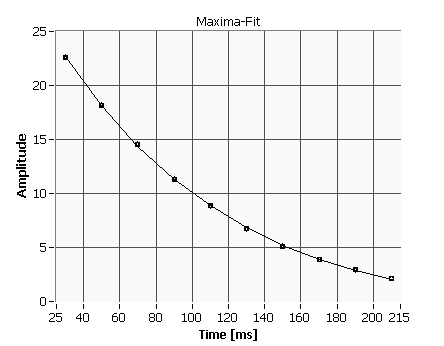
\includegraphics[width=\columnwidth]{graphics/T2_probe1_CP.png}
\captionof{figure}{\small Time evolution of the amplitude of the spin echo of probe 1 measured by Carr-Purcell method}
\label{T2 by CP}
\end{center}

\subsubsection{Magnetic Fields}

The static magnetic field can easily be calculated: $B_0=\frac{\omega_L}{\gamma_I} \approx \frac{2\pi F_p}{\gamma}=\SI{0.466 \pm 0.004}{T}$. The amplitude of the HFP can be derived from the duration of the $90^\circ$- and the $180^\circ$-pulse following $B_1=\frac{\alpha}{\gamma_I \cdot \Delta T}$ which gives us a mean value of $B_1=(4.8\pm 0.2)mT$. Hence, the HFP uses an amplitude of approximately $0.1\%$ of $B_0$.

\newpage

\section{Chemical Shift}

\subsection{Theory and measurement method}

The Larmor frequency $\omega_L$ depends on the total magnetic field $\vec{B}_{tot}$ which is given by the external field $B_0$ and a contribution $\vec{\delta B} = - \sigma \vec{B_0}$ due to the elctron orbitals. The proportionality factor $\sigma$ represents magnetic shielding of $\vec{B_0}$ and charaterises each molecule. By measuring the modified Larmor frequency $\omega_i$ of the sample i, $\sigma_i$ can be determined with the relation $\omega_i = \omega_L (1- \sigma_i)$. To identify different samples the reference substance Tetra-Methyl-Silan (TMS) is added allowing us to measure chemical shifts $\delta_i$ relative to TMS which are defined as $\delta_i = \sigma_i - \sigma_{TMS} = \frac{ \omega_{TMS} - \omega_i }{ \omega_L }$.
Figure \ref{chemical shifts} shows the chemical shifts of organic substances that enabled us to identify unlabeled samples.

\begin{center}
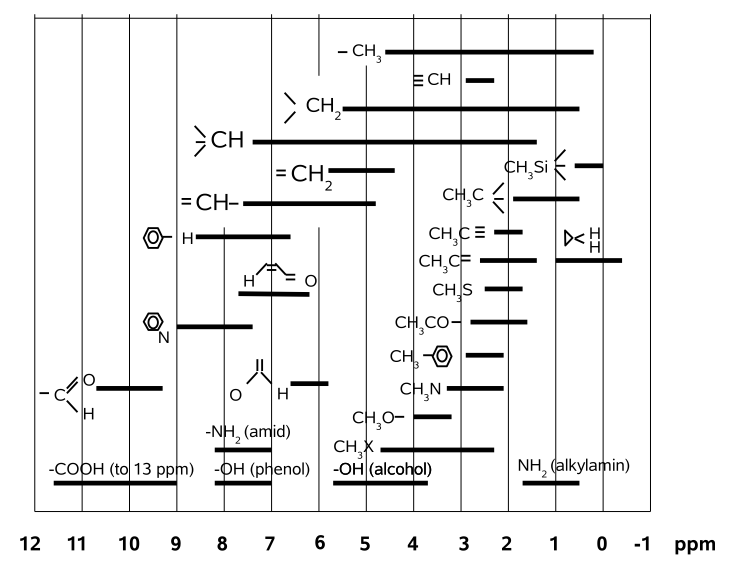
\includegraphics[width=\columnwidth]{graphics/chemical_shifts.png}
\captionof{figure}{\small Chemical shifts $\delta_i$ of different substances}
\label{chemical shifts}
\end{center}

We had to identify the three probes B, C and E. The TMS containing probes were additionally labeled with a "+"-sign.

\subsection{Results}

 We applied a $90^\circ$-pulse to each probe after it had been set into fast rotation. Latter provided that all protons were in average exposed to the same magnetic field despite of its inhomogenity. The Fourier transform of the signal we obtained delivered the "larmor-frequency-spectrum". An example can be seen in the image below.
 
 

\begin{center}
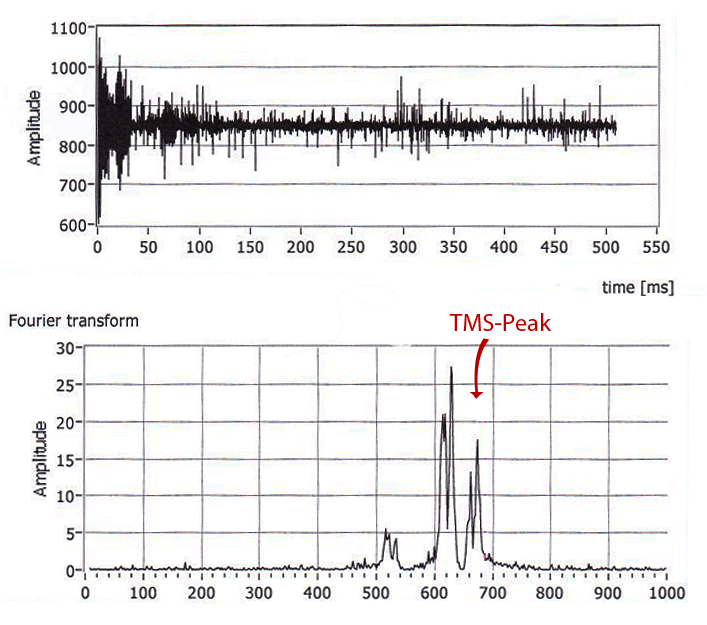
\includegraphics[width=\columnwidth]{graphics/ft.png}
\captionof{figure}{\small Answersignal of probe B+ and its fourier-transform}
\label{probe B}
\end{center}
 
By comparing the characteristic peaks to the TMS-peak we were able to derive the chemmical shift of each substance and came to the following results. This task was simplified as possible solutions were given as Toluol, p-Xylol, acetic acid, fluoracetone and fluoracetonenitrile.

\begin{center}
\begin{tabular}{|c|c|c|}
\hline 
Probe & Shifts & Substance \\ 
\hline 
B & $\delta_1=7.5$; $\delta_2=2.4$ & p-Xylol \\ 
\hline 
C & $\delta_1=10.8$; $\delta_2=2.5$ & acetic acid \\ 
\hline 
E & $\delta_1=7.5$; $\delta_2=2.3$ & Toluol \\ 
\hline 
\end{tabular} 
\end{center}

The high $\delta_1$-shift of probe C (due to the COOH-group) made it easy to identifiy this substance as acetic acid. The shift $\delta_2=2.5$ corresponds to CH$_3$ and verfies our assumption. The shifts of probe B and E were quiet similar and turned out to be p-Xylol or Toluol. As they contain the same chemical groups (benzol and CH$_3$), the two substances can only be distinguished by intensity. P-Xylol contains two of the  CH$_3$-groups and must therefore have a higher peak in the diagramm, which was the case for probe B.

\newpage



\section{1D-Imaging with NMR}

For imaging purposes the magnetic field needs to have a position dependence, typically by gradient fields superimposed to the static field $B_0$. The result is a position depending Larmor frequency allowing us to label the position in the maintained image. 
The first method for one dimensional imaging is called frequency coding. The position of the currently measured Larmor frequency is given as a function of time, whereas phase coding stores the position information within the phase angle of the precessing magnetisation. Both mehtods are mathematically equivalent but differ in the required time for data aquisition.

With these two independent methods we can aquire two dimensional images but only over the full height of the probs. To get two dimensional images at a given intersecting plane a third method is needed: Slice selction. A slice can be selectively excited with a frequency corresponding to the position dependend magnetic field.


\subsection{Results}

To gain information about the gradient-field properties we did seven measurements with water in a glass-tube (fill height: 43mm). The results together with a measurement of 12mm of oil can be seen in the following image:

\begin{center}
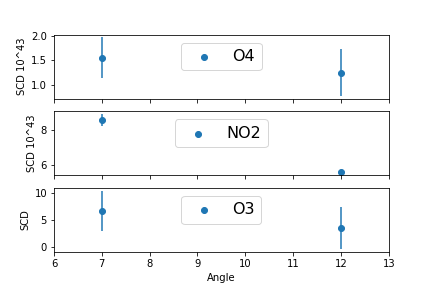
\includegraphics[width=\columnwidth]{SCD_angle.png}
\captionof{figure}{1D-Imaging of water and oil in a glass-tube. The homogenous region of the gradient field reaches from about 0 to 12 mm}
\label{homogenous region}
\end{center}

Obviously the water-probe was "too large" for the spectrometer. It reaches far into the inhomogenous regions of the gradient field. The peaks at the edges show that there the inhomogenousitiy become very strong. The oil probe in contrast was placed almost exactly in the homogenous region of the gradient field. We also recognize that oil has a higher proton-density than water leading to a higher intensity in the waveform. The slope on the right-hand is less steep than on the left-hand. We assume this to be a consequence of the meniscus at the surface.

The next step was to take a 1D-image of a teflon-structure with five layers imersed in oil. In the following image the teflon structure is sketched on the left, the resulting 1D-image is shown on the right.

\begin{center}
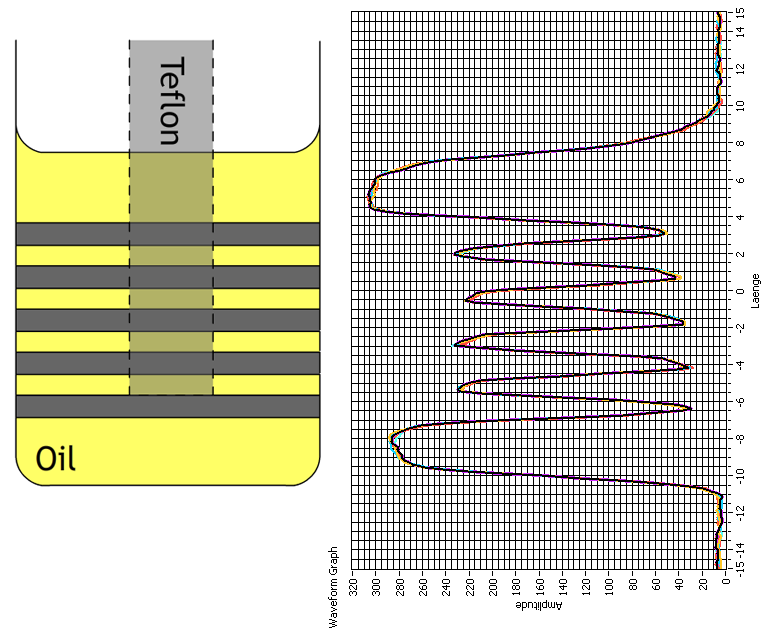
\includegraphics[width=\columnwidth]{graphics/teflon.png}
\captionof{figure}{\small Teflon structure in oil.}
\label{teflon structure}
\end{center}

Teflon does not produce a signal. That the minimums do not equal zero might be caused by little holes inside the teflon slices which allow the oil to pass through or by impurities of the material.

Last we "watched" oil sink into chin-chilla-sand over a longer time period of about 10 minutes.
For the starting setup we put 4mm of oil on top of 15 mm of sand and did 130 scans distributed over the 10 minutes. The following image shows every tenth acquired curve.

\begin{center}
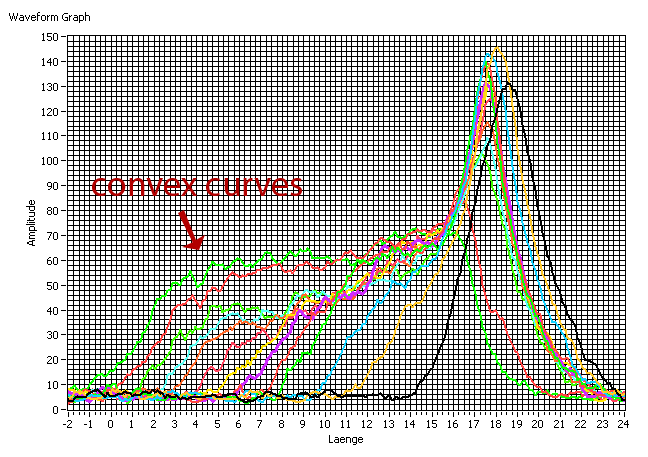
\includegraphics[width=\columnwidth]{graphics/oil_through_sand.png}
\captionof{figure}{\small Oil flowing through sand. The time evolution can be traced from right to left}
\label{oil through sand}
\end{center}

As sand sand does not produce a signal either, the plots directly show the oil sinking deeper and deeper. This process is not a diffusion but driven by gravity. The most obvious arguments for this conclusion are the concave curves on the left-hand side which would have been expected to be convex for a diffusion process.

\section{2D-Imaging with NMR}

With the given spectrometer we were also able to create 2D-images of different objects. The first one is a peanut containing two nuts.

\begin{center}
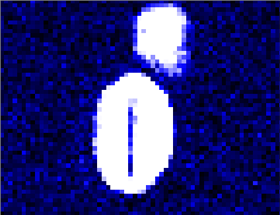
\includegraphics[width=200pt]{graphics/peanut.png}
\captionof{figure}{2\small D-image of a peanut}
\label{peanut}
\end{center}

The shell contains almost no hydrogen, hence it can't be seen on the scan, whereas the nut itself contains lots of oil and delivers a very high signal. We can even observe the air-slit in the middle of the lower nut. 

The last picture is the scan of an olive. The flesh, containing lots of water can be seen clearly.The shell of the kernel delivers no signal therefore appears black just as the stipe channel. The kernel has oil inside which in turn produces a signal.

\begin{center}
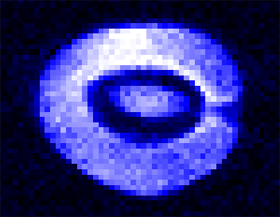
\includegraphics[width=200pt]{graphics/olive.png}
\captionof{figure}{\small Nice picture of an olive}
\label{olive}
\end{center}




\end{multicols}

\end{document}